\section{内核地址空间}

\textbf{地址空间(Address Space)}是一层抽象,在内核中建立虚实地址空间的映射机制,给应用程序提供一个基于地址空间的安全虚拟内存环境,让应用程序简单灵活地使用内存。这层抽象需要达成以下设计目标:
\begin{itemize}
	\item \textbf{透明}:应用开发者可以不必了解底层真实物理内存的硬件细节,且在非必要时也不必关心内核的实现策略,最小化他们的心智负担;
	\item \textbf{高效}:这层抽象至少在大多数情况下不应带来过大的额外开销;
	\item \textbf{安全}:这层抽象应该有效检测并阻止应用读写其他应用或内核的代码、数据等一系列恶意行为。
\end{itemize}

地址空间某种程度上讲,可以将它看成一块巨大但并不一定真实存在的内存。在每个应用程序的视角里,操作系统分配给应用程序一个地址范围受限(容量很大),独占的连续地址空间(其中有些地方被操作系统限制不能访问,如内核本身占用的虚地址空间等),因此应用程序可以在划分给它的地址空间中随意规划内存布局,它的各个段也就可以分别放置在地址空间中它希望的位置(当然是操作系统允许应用访问的地址)。

由于每个应用独占一个地址空间,里面只含有自己的各个段,于是它可以随意规划属于它自己的各个段的分布而无需考虑和其他应用冲突;同时鉴于应用只能通过虚拟地址读写它自己的地址空间,它完全无法窃取或者破坏其他应用的数据,毕竟那些段在其他应用的地址空间内,这是它没有能力去访问的。这是地址空间抽象和具体硬件机制对应用程序执行的安全性和稳定性的一种保障。

在本章之前,内核和应用代码的访存地址都被视为一个物理地址,并直接访问物理内存,而在分页模式开启之后,CPU先拿到虚存地址,需要通过 MMU 的地址转换变成物理地址,再交给 CPU 的访存单元去访问物理内存。地址空间抽象的重要意义在于 \textbf{隔离 (Isolation)},当内核让应用执行前,内核需要控制 MMU 使用这个应用的多级页表进行地址转换。由于每个应用地址空间在创建的时候也顺带设置好了多级页表,使得只有那些存放了它的代码和数据的物理页帧能够通过该多级页表被映射到,这样它就只能访问自己的代码和数据而无法触及其他应用或内核的内容。

启用分页模式下,内核代码的访存地址也会被视为一个虚拟地址并需要经过 MMU 的地址转换,因此我们也需要为内核对应构造一个地址空间,它除了仍然需要允许内核的各数据段能够被正常访问之后,还需要包含所有应用的内核栈以及一个跳板 (Trampoline)。

\subsection{内核虚拟地址空间分布}

内核虚拟地址空间分布是计算机操作系统中的一个重要概念。在操作系统中,虚拟地址空间是指用户程序所访问的内存空间,它与物理内存空间不同,它是一个虚拟的地址空间。内核虚拟地址空间分布是指内核中的进程管理、内存管理和文件系统等模块所使用的虚拟地址空间的布局和结构。

在计算机系统中,内核虚拟地址空间分布的合理安排可以提高系统的性能。例如,当用户程序需要访问内存中的数据时,如果内存空间不足,系统就需要将数据复制到更多的内存中,这会增加系统的开销。但如果内核虚拟地址空间分布合理,可以将部分数据缓存在磁盘上,从而减少内存空间的占用,提高系统的性能。

因此,了解内核虚拟地址空间分布的基本知识对于我们来讲是非常重要的。本文将介绍内核虚拟地址空间分布的基本概念、组织结构和使用方法,以便读者更好地理解内核虚拟地址空间分布的重要性和作用。

在操作系统中,内核空间通常被划分为多个不同的区域,这些区域用于存储不同的数据结构和代码。以下是一些常见的内核空间划分:
\begin{itemize}
	\item \textbf{代码段 (Code Segment)}:代码段用于存储内核代码,包括系统调用接口、中断处理程序、内核函数等。代码段通常被标记为只读,并且只能在内核编译时进行分配。
	\item \textbf{数据段 (Data Segment)}:数据段用于存储内核数据和变量,包括进程管理数据、内存管理数据、网络数据等。数据段通常可以被内核修改。
	\item \textbf{堆栈段 (Stack Segment)}:堆栈段用于存储进程的栈数据,包括函数调用堆栈、参数传递堆栈等。堆栈段通常被标记为只读,并且只能在内核编译时进行分配。
	\item \textbf{全局变量段 (Global Variable Segment)}:全局变量段用于存储全局变量和静态变量。全局变量段通常可以被内核修改。
	\item \textbf{中断向量表 (Interrupt Vector Table)}:中断向量表用于存储内核中的中断处理程序地址。中断向量表通常被标记为只读,并且只能在内核编译时进行分配。
	\item \textbf{内核引导段 (Kernel Boot Segment)}:内核引导段用于存储内核引导程序,用于启动操作系统。内核引导段通常被标记为只读,并且只能在内核编译时进行分配。
\end{itemize}

在内核编译时,通常会根据内核的功能和需求进行空间分配,以确保内核能够正确运行。不同的内核版本可能会有不同的空间分配策略,但通常需要考虑内存使用、代码和数据的可读性和可维护性等因素。

不同的内核有不同的地址空间划分,并找不到一种通用的划分, 如下图 \ref{内核虚拟地址空间分布},我们可以看到NPUcore 的内核虚拟地址空间分布图:
\begin{figure}[h]
	\centering
	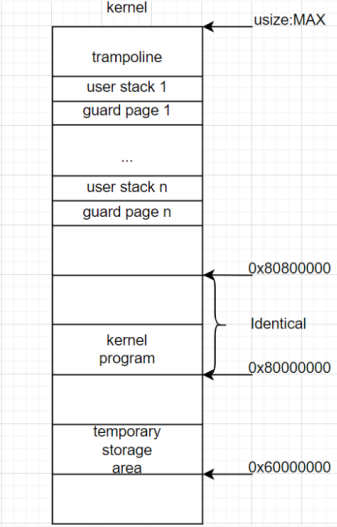
\includegraphics[width=0.3\textwidth]{figures/04-02-内核虚拟地址空间分布.png}
	\caption{内核虚拟地址空间分布}
	\label{内核虚拟地址空间分布}
\end{figure}

\begin{itemize}
	\item \textbf{trampoline}:跳板(trampoline),跳板页面的大小是 1 page,这个页面在地址空间的最高虚拟页面上。在内核空间中,跳板唯一的用途就是发生 panic。
	\item \textbf{user stack}:接下来则是从高到低放置用户栈,栈向下增长。每个user stack的大小为 1 page。
	\textbf{用户栈 (User Stack)}是操作系统中的一种数据结构,用于存储用户程序执行期间所需的临时数据和指令。用户栈通常位于系统的虚拟内存中,是一个固定大小的数组,用于存储程序运行期间的临时数据和指令。在程序运行时,操作系统会为程序创建一个用户栈,用于存储程序执行期间的临时数据和指令。这些数据和指令包括程序运行时需要的临时变量、函数调用时的返回地址、参数等。当程序执行完毕后,操作系统会将该栈中的数据清除,以便为新的程序运行提供空间。
	
	用户栈的基本概念包括栈帧、栈空间、栈底和栈顶等,这些概念对于理解程序的执行过程和程序的内存分布非常重要。需要注意的是这里的userstack并不专指用户栈,当某个进程处于S模式时,内核将使用此区域作为内核堆栈。
	\item \textbf{guard page}:相邻两个内核栈之间会预留一个 保护页面 (Guard Page),页面大小也是 1 page。这些页面位于堆栈页面之下。它们未被分配,这意味着如果内核使用这些区域中的数据,将捕获页面错误。它们保护内核不修改另一个进程的堆栈数据。
	用户栈的基本概念包括:
	
	\begin{enumerate}
		\item 栈帧 (Stack Frame):栈帧是用户栈中的数据结构,用于存储程序运行时所需的临时数据和指令。每个栈帧都包含一个返回地址 (Return Address) 和一个数据区 (Data Area),其中数据区用于存储程序运行期间的临时数据和指令。
		\item 栈空间 (Stack Space):栈空间是用户栈中的数据结构,用于存储程序运行时所需的临时数据和指令。栈空间的大小通常由操作系统分配和回收,程序运行时所需的栈空间大小由程序控制。
		\item 栈底 (Stack Bottom):栈底是用户栈中的数据结构,用于表示当前栈中存储的数据和指令的起始地址。栈底通常是程序运行时的数据构,用于存储程序的返回地址和参数等。
		\item 栈顶 (Stack Top):栈顶是用户栈中的数据结构,用于表示当前栈中存储的数据和指令的结束地址。栈顶通常是程序运行时的数据结构,用于存储程序的返回地址和参数等。
		\item 入栈 (Push):入栈是将数据或指令压入用户栈中的数据结构中。入栈的操作通常用于将数据或指令存储到栈中,以便程序在执行时能够访问这些数据或指令。
		\item 出栈 (Pop):出栈是将栈中的数据或指令弹出到程序的数据结构中。出栈的操作通常用于将数据或指令从栈中弹出,以便程序在执行时能够访问这些数据或指令。
	\end{enumerate}
	
	由于编译器会对访存顺序和局部变量在栈帧中的位置进行优化,我们难以确定一个已经溢出的栈帧中的哪些位置会先被访问,但总的来说,保护页面大小被设置的越大,我们就能越早捕获到这一可能覆盖其他重要数据的错误异常。由于我们的内核非常简单且内核栈的大小设置比较宽裕,在当前的设计中我们仅将其大小设置为单个页面。
	\item \textbf{kernel program}:这里将加载内核程序。注意到这里有 identical 标识,表明这段空间是恒等映射,之后会在内核物理空间详细介绍。
	\item \textbf{temporary storage area}:临时存储区域,这个区域最多占据 512 pages。这个区域现在用于exec系统调用,这意味着文件将首先加载到这里。
\end{itemize}

\subsection{内核物理地址空间分布}

在计算机系统中,内核物理地址空间分布是一个非常重要的概念。它决定了计算机系统如何访问内存
和其他硬件资源,并且是操作系统和内核中的一个重要概念。下面将介绍内核物理地址空间分布的基本概
念和原理,并提供一些常见的应用场景。

在计算机系统中,物理地址空间是一个固定的物理内存地址范围,用于存储操作系统和内核中的各种
数据结构和代码。虚拟地址空间是一个虚拟的内存地址范围,它被操作系统和内核映射到物理地址空间中。内核物理地址空间分布是指在虚拟地址空间中,内核所占用的物理内存地址范围。

内核物理地址空间分布通常被划分为多个不同的区域,这些区域用于存储不同的数据结构和代码。例如,代码段、数据段、堆栈段、全局变量段等,这些区域的大小和位置都会在内核编译时进行分配。在内核物理地址空间分布中,还有一些特殊的区域,如内核引导段和中断向量表等,这些区域用于存储内核引导程序和中断处理程序的地址。

内核物理地址空间分布的基本概念和原理对于操作系统和内核的设计和实现⾮常重要。了解内核物理地址空间分布的基本概念和原理可以帮助我们更好地设计和实现操作系统和内核,从而提高系统的可靠性和性能。此外,内核物理地址空间分布的基本概念和原理也可以应用于其他计算机系统的设计和实现中。

\subsubsection{内核程序区域}

在Memoryset的new\_kernel()方法中,首先map了trampoline(这里不是恒等映射,trampoline虽然在虚拟地址的最顶端,但是物理地址并没有到那么高),由anonymous\_identical\_map!匿名恒等映射宏可知,接下来恒等映射内核的四个逻辑段.text .rodata . data和 .bss。最后恒等映射 physical memory和 memory-mapped registers。

之所以使用恒等映射到物理内存的方法,是因为这能够使得我们在无需调整内核内存布局os/src/linker-xxx.ld 的情况下,仍能像启用页表机制之前那样访问内核的各个段。

在内核运行时会输出如下内容:

\begin{lstlisting}[language={Rust}]
	.text [0x80200000, 0x80237000)
	.rodata [0x80237000, 0x80240000)
	.data [0x80240000, 0x80241000)
	.bss [0x80241000, 0x80492000)
	mapping .text section
	mapping .rodata section
	mapping .data section
	mapping .bss section
	mapping physical memory
	mapping memory-mapped registers
\end{lstlisting}

上述输出的内容对应创建内核地址空间的方法new\_kernel的代码。不同字段的作用如下:

\begin{itemize}
	\item[$\bullet$] .text
	
	代码段,存放需要执行的代码,该空间拥有读权限和执行权限。
	
	\item[$\bullet$] .rodata
	
	只读数据段,存放只读数据,该空间拥有读权限。
	
	\item[$\bullet$] .data
	
	数据段,该空间拥有读权限和写权限。要想辨别其与.rodata的区别,下面的C语言示例可以帮助我们更好地理解
	
	\begin{lstlisting}[language={C}]
		int bss_value1=5;//全局的被初始化的变量,存放于data段
		const int cbss_value1=5;//加上const变为只读的常量,存放于rodata段
	\end{lstlisting}
	
	\item[$\bullet$] .bss
	
	⽤来存储一些未被初始化的全局变量和静态变量的内存区域,一般在初始化时.bss段部分将会清零。不包含任何数据,只是简单的维护开始和结束的地址,以便内存区能在运行时被有效地清零。可以被读写,但不允许从它上面取指执行。
	
\end{itemize}


\hspace*{\fill}

不同区域读写执行权限不同是通过 MapPermission 映射区域的权限来控制的,标志如下:
\begin{lstlisting}[language={Rust}]
	//os/src/mm/memory_set.rs
	
	bitflags! {
		pub struct MapPermission: u8 {
			const R = 1 << 1;// 读
			const W = 1 << 2;// 写
			const X = 1 << 3;// 执⾏
			const U = 1 << 4;// 用户
		}
	}
\end{lstlisting}

字段地址确定首先要通过外部符号的引用,引入这些标记是为了在下面恒等映射中引用,确定恒等映射的地址区域。下面是extern "C" 的引用:
\begin{lstlisting}[language={Rust},caption={extern "C"}]
	//os/src/mm/memory_set.rs
	extern "C" {
		fn stext();
		fn etext();
		fn srodata();
		fn erodata();
		fn sdata();
		fn edata();
		fn sbss_with_stack();
		fn ebss();
		fn ekernel();
		fn strampoline();
		fn ssignaltrampoline();
	}
\end{lstlisting}
从 os/src/linker-xxx.ld 中引用了很多表示各个段位置的符号。可以看到在 os/src 目录下有三个 ld 文件: linker-qemu.ld , linker-k210.ld , linker-fu740.ld ,分别对应 qemu , k210 和 fu740 三个平台。其实三者只有第三行的 BASE\_ADDRESS 不同, k210 为 0x80020000 , qemu 与 fu740 均为 0x80200000 。

此外还有\textbf{physical memory}(物理内存),内核地址空间中需要存在一个恒等映射到内核数据段之外的可用物理页帧的逻辑段,这样才能在启用页表机制之后,内核仍能以纯软件的方式读写这些物理页帧。

有了以上的知识,可以画出这五段逻辑区域的物理地址空间分布如下图 \ref{逻辑区域的物理地址空间分布}:
\begin{figure}[htb]
	\centering
	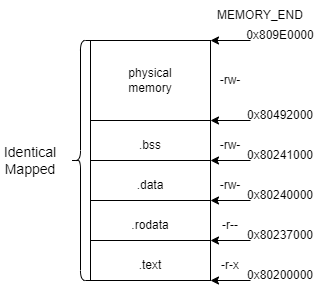
\includegraphics[width=0.5\linewidth]{figures/04-02-逻辑区域的物理地址空间.png}
	\caption{
		逻辑区域的物理地址空间分布
	}
	\label{逻辑区域的物理地址空间分布}
\end{figure}


需要特别说明的是,这里画出的只是在 qemu 平台上的地址空间分布,在 k210 或 fu740 上则不一样。一是因为上⽂提到 k210 的 BASE\_ADDRESS 为 0x80020000 ,不同于 qemu 的 0x80200000 。二是因为 MEMORY\_END 在不同平台上也不相同,具体如下:
\begin{lstlisting}[language={Rust},caption={config.rs}]
	//os/src/config.rs
	#[cfg(all(not(feature="board\_k210"), not(feature="board\_fu740")))]
	pub const MEMORY_END: usize = 0x809e_0000;
	#[cfg(feature = "board_k210")]
	pub const MEMORY_END: usize = 0x8080_0000;
	#[cfg(feature = "board_fu740")]
	pub const MEMORY_END: usize = 0x9000_0000;
\end{lstlisting}

\subsubsection{内存映射空间}

\textbf{MMIO}(Memory-mapped
I/O,即内存映射I/O),通过将外围设备映射到内存空间,便于CPU的访问。
使用这种处理方式,设备控制寄存器只是内存中的变量,可以和其他变量一样进行寻址,无需特殊的I/O指令(如 IN , OUT)来读写设备控制器。而且这种⽅式可以将设备的读取权限管理同区域读取权限管理结合起来,这个区域没有 U 权限标志,那么就只可以在内核态被访问,无需特殊的保护机制。

\begin{lstlisting}[language={Rust}, caption={//os/board}]
	//os/src/boards/qemu.rs
	pub const MMIO: &[(usize, usize)] = &[
	(0x1000_0000, 0x1000),
	(0x1000_1000, 0x1000),
	(0xC00_0000, 0x40_0000),
	];
	//os/src/boards/fu740.rs
	pub const MMIO: &[(usize, usize)] = &[
	(0x1000_0000, 0x1000), // PRCI
	(DISK_IMAGE_BASE, 0x800_0000), // disk image
	];
	//os/src/boards/k210.rs
	pub const MMIO: &[(usize, usize)] = &[
	// we don't need clint in S priv when running
	// we only need claim/complete for target0 after initializing
	(0x0C00_0000, 0x3000), /* PLIC */
	(0x0C20_0000, 0x1000), /* PLIC */
	(0x3800_0000, 0x1000), /* UARTHS */
	(0x3800_1000, 0x1000), /* GPIOHS */
	(0x5020_0000, 0x1000), /* GPIO */
	(0x5024_0000, 0x1000), /* SPI_SLAVE */
	(0x502B_0000, 0x1000), /* FPIOA */
	(0x502D_0000, 0x1000), /* TIMER0 */
	(0x502E_0000, 0x1000), /* TIMER1 */
	(0x502F_0000, 0x1000), /* TIMER2 */
	(0x5044_0000, 0x1000), /* SYSCTL */
	(0x5200_0000, 0x1000), /* SPI0 */
	(0x5300_0000, 0x1000), /* SPI1 */
	(0x5400_0000, 0x1000), /* SPI2 */
	];
\end{lstlisting}
其中每个元组的第一个数为起始地址,第二个数为区域大小。据此来分配 MMIO
,权限均为可读可写。在 new\_kernel() 方法中对应的映射代码为:
\begin{lstlisting}[language={Rust},	caption={//os/mm/memory\_set.rs}]
	macro_rules! anonymous_identical_map {
		($begin:expr,$end:expr,$permission:expr) => {
			memory_set
			.push(
			MapArea::new(
			($begin as usize).into(),
			($end as usize).into(),
			MapType::Identical,
			$permission,
			None,
			),
			None,
			)
			.unwrap();
		};
		($name:literal,$begin:expr,$end:expr,$permission:expr) => {
			println!("mapping {}", $name);
			anonymous_identical_map!($begin, $end, $permission);
		};
	}   
	
	println!("mapping memory-mapped registers");
	for pair in MMIO {
		anonymous_identical_map!(
		(*pair).0,
		((*pair).0 + (*pair).1),
		MapPermission::R | MapPermission::W
		);
	}
\end{lstlisting}

该函数用于将 MMIO 内存区域恒等映射到物理内存中。MMIO
内存区域通常⽤于存储设备驱动程序的缓冲区,这些缓冲区需要被映射到进程的虚拟内存地址空间中,以便进程可以访问它们。

在这段代码中, MMIO 是一个枚举类型,它定义了 MMIO
内存区域的权限和起始地址。 \texttt{anonymous\_identical\_map!}
是一个匿名函数,用于做恒等内存映射。该函数接受三个参数:一个起始地址、一个终止地址、以及一个映射权限。在本例中,
\texttt{(*pair).0} 和 \texttt{(*pair).1} 分别表示 MMIO 内存区域的起始地址和长度,
\texttt{MapPermission::R\ \textbar{}\ MapPermission::W}
表示读取和写入权限。 函数的循环遍历了 MMIO
枚举类型中的所有内存区域,并为每个区域做恒等映射。在创建每个映射时,函数使用了 \texttt{anonymous\_identical\_map!} 函数,以便为每个区域做恒等映射,这些映射空间具有相同的权限。

\subsubsection{地址空间实现}

在前面,我们介绍了地址空间的概念层面,描述了地址空间的分布和映射关系。接下来,我们将深入NPUcore内部,探讨地址空间这一抽象概念在NPUcore中的实现。

首先,从数据结构入手。地址空间由页表和一系列内存映射区域构成。在NPUcore中,页表可以直接创建为PageTable对象,而内存映射区域需要使用一个MapArea的向量(vec)来表示。具体代码如下:

\begin{lstlisting}[language={Rust}, caption={MemorySet}]
	pub struct MemorySet {
		page_table: PageTable,
		/// The mapped area.
		/// Segments are implemented using this mechanism. In other words, they may be considered a subset of MapArea.
		/// Yet, other purposes may exist in this struct, such as file mapping.
		areas: Vec<MapArea>,
	}
\end{lstlisting}
有关多级页表的具体实现将在后续章节详细讲解。这里我们主要关注MapArea的实现:

\begin{lstlisting}[language={Rust},caption={MapArea}]
	#[derive(Clone)]
	/// Map area for different segments or a chunk of memory for memory mapped file access.
	pub struct MapArea {
		/// Range of the mapped virtual page numbers.
		/// Page aligned.
		/// Map physical page frame tracker to virtual pages for RAII & lookup.
		inner: LinearMap,
		/// Direct or framed(virtual) mapping?
		map_type: MapType,
		/// Permissions which are the OR of RWXU, where U stands for user.
		map_perm: MapPermission,
		pub map_file: Option<Arc<dyn File>>,
	}
	
	#[derive(Copy, Clone, PartialEq, Debug)]
	pub enum MapType {
		Identical,
		Framed,
	}
\end{lstlisting}
MapPermission表示映射权限,MapType表示映射方式,分为直接映射(Identical)和间接映射(Framed)。inner是一种LinearMap类型,表示MapArea所映射到的内存区域,其实现如下:

\begin{lstlisting}[language={Rust}, caption={LinearMap}]
	#[cfg(not(feature = "oom_handler"))]
	#[derive(Clone)]
	pub struct LinearMap {
		vpn_range: VPNRange,
		frames: Vec<Frame>,
	}
\end{lstlisting}
VPNRange表示虚拟页号的范围,通过VPNRange可以了解到该内存区域的大小。frames是枚举类型Frame的向量。关于Frame的枚举类型的具体代码如下:

\begin{lstlisting}[language={Rust}, caption={Frame}]
	pub enum Frame {
		InMemory(Arc<FrameTracker>),
		Unallocated,
	}
	
	pub struct FrameTracker {
		pub ppn: PhysPageNum,
	}
\end{lstlisting}

这里利用枚举类型对FrameTracker做了一个封装,FrameTracker绑定每个物理页面,作为物理页面跟踪器。将物理页追踪器映射到虚拟页面有利于RAII和进行页面查找。

RAII(Resource Acquisition Is Initialization),也称为“资源获取就是初始化”,简单地说,RAII的做法是使用一个对象,在其构造时获取资源,在对象生命周期内控制对资源的访问,使之始终保持有效,最后在对象析构的时候释放资源。

在这里就是使FrameTracker与物理页面有相同的生命周期,当获取物理页面构建FrameTracker时就将物理页面初始化,在释放FrameTracker时也将自动回收物理页面。具体见以下代码:

\begin{lstlisting}[language={Rust}, caption={FrameTracker}]
	impl FrameTracker {
		pub fn new(ppn: PhysPageNum) -> Self {
			// page cleaning
			let dwords_array = ppn.get_dwords_array();
			for i in dwords_array {
				*i = 0;
			}
			Self { ppn }
		}
		
		pub unsafe fn new_uninit(ppn: PhysPageNum) -> Self {
			Self { ppn }
		}
	}
	
	impl Drop for FrameTracker {
		/// Automatically recycle the physical frame when
		fn drop(&mut self) {
			// println!("do drop at {}", self.ppn.0);
			frame_dealloc(self.ppn);
		}
	}
\end{lstlisting}

需要说明的是FrameTracker的生命周期也被一层层绑定到它所在的逻辑段MapArea下,当逻辑段被回收之后这些之前分配的物理页帧也会自动地同时被回收。同理,MapArea的生命周期也随着MemorySet,这样就做到了当一个地址空间MemorySet生命周期结束后,这些物理页帧都会被回收。
接下来分析几个MemorySet接口下常用方法:

创建内核地址空间的方法new\_kernel。具体创建方式在前面章节已经给出。这里给出该函数下调用的其他与MemorySet相关的函数:

\begin{lstlisting}[language={Rust}, caption={内核创建}]
	MemorySet
	├── new_bare()// 新建一个空的地址空间
	├── new_kernel()// 新建一个空的内核空间,在前面介绍过
	├── map_trampoline()// 映射跳板区域
	├── push()// 将MapArea push 到MemorySet 中
	└── MapArea
	├── map_one()// 映射页面前的检查,检查完调用下面的方法
	└── map_one_unchecked()// 映射页面的具体实现
\end{lstlisting}
首先调用的是new\_bare函数,其作用是创建一个空的

页表和空的areas向量,具体实现如下:

\begin{lstlisting}[language={Rust}, caption={new\_bare}]
	impl MemorySet {
		/// Create a new struct with no information at all.
		pub fn new_bare() -> Self {
			Self {
				page_table: PageTable::new(),
				areas: Vec::with_capacity(16),
			}
		}
	}
\end{lstlisting}

之后首先映射跳板区域,注意这个跳板区域并没有被包括在areas里。
\begin{lstlisting}[language={Rust}, caption={trampoline}]
	fn map_trampoline(&mut self) {
		self.page_table.map(
		VirtAddr::from(TRAMPOLINE).into(),
		PhysAddr::from(strampoline as usize).into(),
		PTEFlags::R | PTEFlags::X,
		);
	}
\end{lstlisting}

物理地址是通过extern "C"引用的外部符号strampoline,TRAMPOLINE被设置为最高虚拟页。跳板页面存放的是可执行的代码,权限是读与执行。

其余区域的映射方式大致相同,NPUcore定义了一个anonymous\_identical\_map宏(匿名恒等映射),来减少重复代码。具体代码如下:

\begin{lstlisting}[language={Rust},  caption={anonymous\_identical\_map}]
	macro_rules! anonymous_identical_map {
		($begin:expr,$end:expr,$permission:expr) => {
			memory_set
			.push(
			MapArea::new(
			($begin as usize).into(),
			($end as usize).into(),
			MapType::Identical,
			$permission,
			None,
			),
			None,
			)
			.unwrap();
		};
		($name:literal,$begin:expr,$end:expr,$permission:expr) => {
			println!("mapping {}", $name);
			anonymous_identical_map!($begin, $end, $permission);
		};
	}
\end{lstlisting}
这个宏有两个分支。四个参数时,第一个参数为被map的区域名称,会被打印一下再调用三个参数的分支。三个参数时,分别为起始地址,终止地址和映射区域的权限。注意在MapArea::new中有MapType::Identical,这个决定了调用这个宏的映射都是恒等映射。这个宏主体部分调用了MemorySet的push方法:

\begin{lstlisting}[language={Rust}, caption={push}]
	fn push(&mut self, mut map_area: MapArea, data: Option<&[u8]>) -> Result<(), MemoryError> {
		match data {
			Some(data) => {
				let mut start = 0;
				let len = data.len();
				for vpn in map_area.inner.vpn_range {
					let ppn = map_area.map_one(&mut self.page_table, vpn)?;
					let end = start + PAGE_SIZE;
					let src = &data[start..len.min(end)];
					ppn.get_bytes_array()[..src.len()].copy_from_slice(src);
					start = end;
				}
			}
			None => {
				for vpn in map_area.inner.vpn_range {
					map_area.map_one(&mut self.page_table, vpn)?;
				}
			}
		}
		self.areas.push(map_area);
		Ok(())
	}
\end{lstlisting}

方法的功能是,将尚未映射的MapArea push到当前MemorySet中,并为映射分配所需的内存,如果没有数据,那么直接遍历map\_area.inner.vpn\_range(虚拟页面页号),使用MapArea的map\_one方法来映射每个页面。如果有数据的话,在上述操作之外还需添加将数据拷贝映射后的物理页面的操作。
下面看一下map\_one方法的实现:

\begin{lstlisting}[language={Rust}, caption={map\_one}]
	pub fn map_one(
	&mut self,
	page_table: &mut PageTable,
	vpn: VirtPageNum,
	) -> Result<PhysPageNum, MemoryError> {
		if !page_table.is_mapped(vpn) {
			//if not mapped
			Ok(self.map_one_unchecked(page_table, vpn))
		} else {
			//mapped
			Err(MemoryError::AlreadyMapped)
		}
	}
	
	pub fn map_one_unchecked(
	&mut self,
	page_table: &mut PageTable,
	vpn: VirtPageNum,
	) -> PhysPageNum {
		let ppn: PhysPageNum;
		match self.map_type {
			MapType::Identical => {
				ppn = PhysPageNum(vpn.0);
			}
			MapType::Framed => {
				let frame = unsafe { frame_alloc_uninit().unwrap() };
				ppn = frame.ppn;
				self.inner.alloc_in_memory(vpn, frame);
			}
		}
		let pte_flags = PTEFlags::from_bits(self.map_perm.bits).unwrap();
		page_table.map(vpn, ppn, pte_flags);
		ppn
	}
\end{lstlisting}

map\_one首先会检查传入的vpn是否已经被分配,如已经分配会报错MemoryError::AlreadyMapped,未分配移交给map\_one\_unchecked来分配。分配时会根据分配类型来分别处理,如为Identical则物理地址与虚拟地址恒等映射,如为Framed则会申请一个空闲物理页面(frame\_alloc\_uninit)与之映射(page\_table.map)。

在整个代码中,对NPUcore地址空间的实现进行了清晰的分层和结构化设计,采用了合理的数据结构和接口设计,实现了对虚拟地址空间的灵活管理。